\subsubsection{分析与准备：必要条件对应观测证据}

多光束判定须分清形成、计算、观测与测厚影响。非零界面返回、时间相干、空间重叠与仪器分辨四类条件缺一不可；两个界面存在只涉及首项。

往返复倍率即每轮返回场的共同衰减与相位因子。其最大模（幅度比例）在硅两次留段为$0.1333$和$0.0769$，碳化硅为$0.0258$和$0.0076$，均无量纲；图\ref{fig:roundtrip}中的光路说明相邻返回为何乘以同一复数，收敛与实验观测由不同条件控制。
% src:求解/问题3/结果/公平对照.json:案例.1.场级数核验.最大往返乘子模;案例.2.场级数核验.最大往返乘子模;案例.4.场级数核验.最大往返乘子模;案例.5.场级数核验.最大往返乘子模

\begingroup
\setlength{\intextsep}{2pt}
\begin{figure}[H]
  \centering
  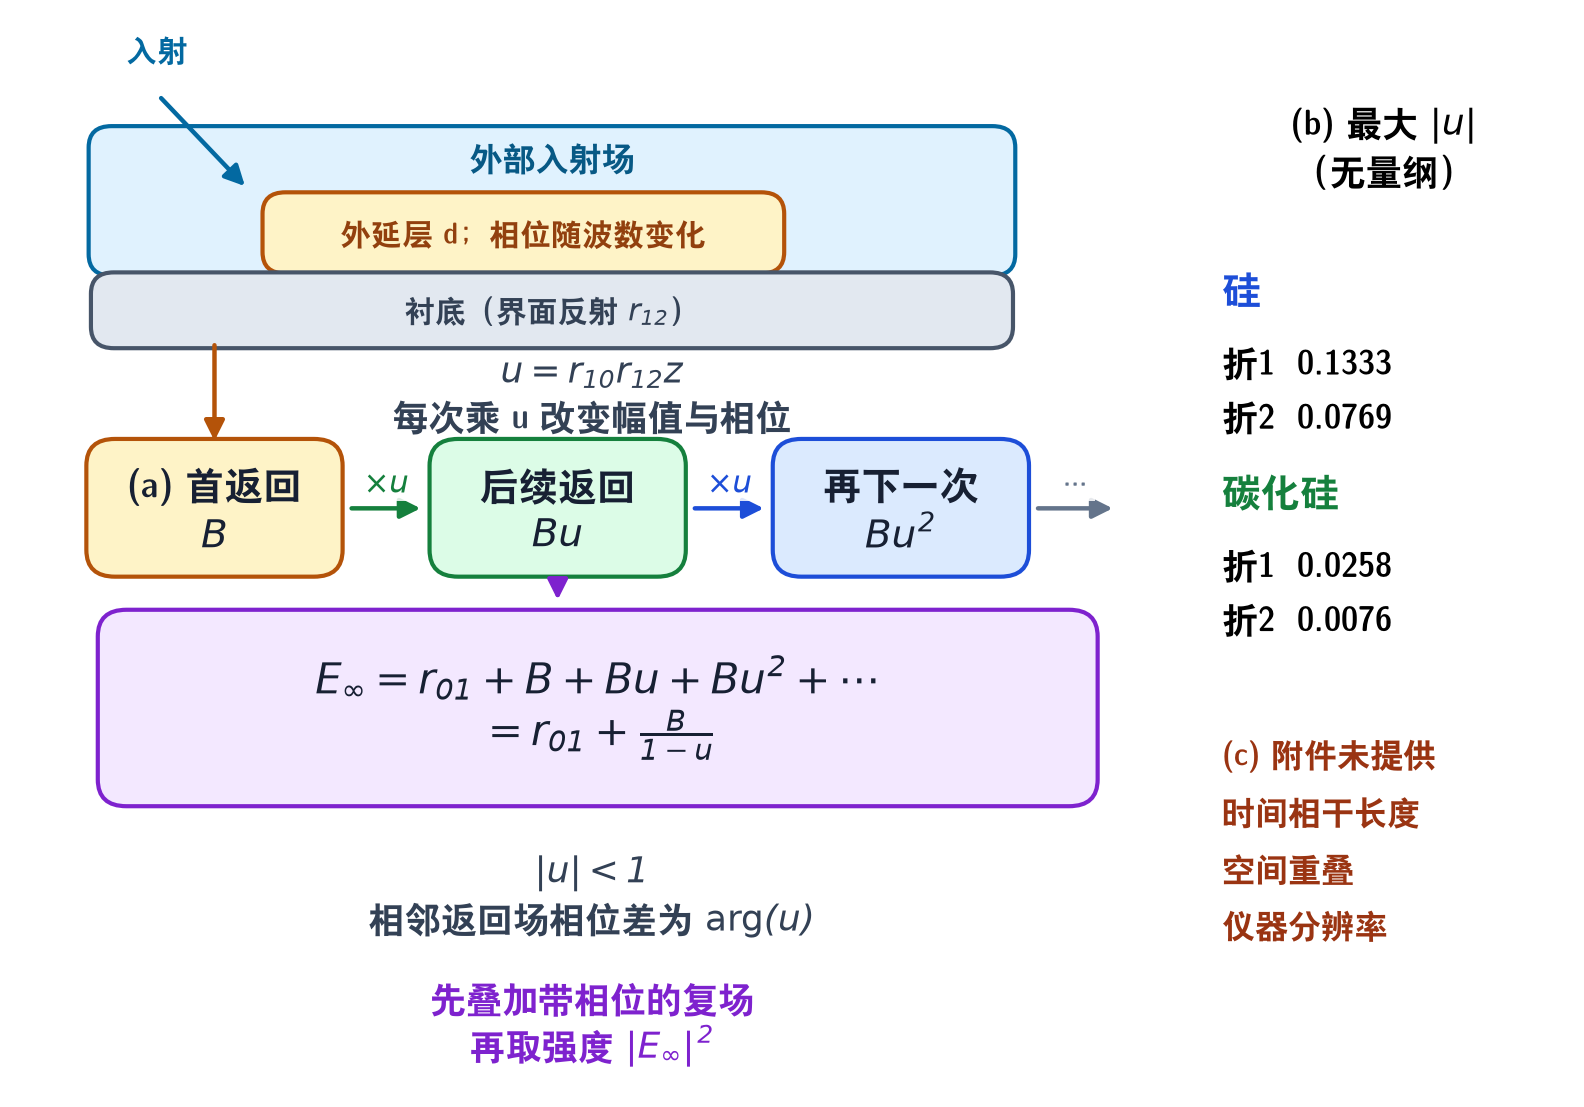
\includegraphics[width=0.96\textwidth]{../求解/问题3/图片/多次往返按复振幅递减.png}
  \caption{返回光的复振幅随往返次数递减}
  \label{fig:roundtrip}
\end{figure}
\endgroup

逐项核对发现，硅双角原始相关系数虽达$0.9943$，相干、重叠及分辨资料却均缺失，因而排除高相关直接判定；表\ref{tab:07}把已知量与未知量分列。
% src:交接/数据档案.json:跨文件关系.两两全量核验.5.原始反射率皮尔逊相关系数
% src:交接/实验记录.json:547.尝试;547.现象;547.决定

\begingroup
\footnotesize
\setlength{\LTpre}{3pt}
\setlength{\LTpost}{3pt}
\begin{longtable}{>{\centering\arraybackslash}p{0.16\textwidth} >{\centering\arraybackslash}p{0.18\textwidth} >{\centering\arraybackslash}p{0.17\textwidth} >{\centering\arraybackslash}p{0.16\textwidth} >{\centering\arraybackslash}p{0.17\textwidth}}
\caption{多光束必要条件与四附件证据}\label{tab:07}\\
\hline
必要条件 & 核对对象 & 四附件已有信息 & 缺失信息 & 替代解释\\
\hline
界面返回 & 界面反射系数 & 模型可核验 & 实测光学常数 & 界面弱反射\\
时间相干 & 往返相位关联 & 均未给资料 & 相干长度 & 相位随机化\\
空间重叠 & 返回光束重合 & 均未给资料 & 光路、偏振 & 光束错位\\
仪器分辨 & 高阶谱形差 & 反射率均已给 & 分辨率、噪声 & 基线与色散\\
\hline
\end{longtable}
\endgroup
% src:求解/问题3/结果/条件判定.json:必要条件
% src:交接/数据档案.json:未随附件提供的建模输入

慢变基线也可抬高相关；折射率随波数的变化称为色散，也会改变谱形。故两束截断场与完整往返场采用同波段、同训练及留出区段、同基线复杂度，逐角评价谱形相容性。下一节沿此对照推导有限往返及收敛闭式，再讨论厚度影响。
